\documentclass{article}
\usepackage{amsmath}
\usepackage{mathtools}
\usepackage{gensymb}
\usepackage[a4paper,inner=1.5cm,outer=1.5cm,top=2cm,bottom=0.5cm]{geometry} 
\usepackage{xcolor}                    
\usepackage{tikz}                           
\usepackage{multicol}
\usepackage{pgfplots}
\usetikzlibrary{calc}
\usetikzlibrary{intersections}
\usetikzlibrary{intersections,calc,angles,quotes}
\usetikzlibrary{shapes,arrows,positioning,decorations.pathreplacing,calc}
\usetikzlibrary{calc,angles,positioning,intersections,quotes,decorations.markings}
\usepackage{tkz-euclide}
\usetikzlibrary{backgrounds}
\usetikzlibrary{calc,through}
\usetikzlibrary{angles}
\usetikzlibrary{fadings}
\usetikzlibrary{shapes.geometric}
\usetikzlibrary{shapes.symbols}
\usepackage{draftwatermark}
\usepackage{mathptmx}

\SetWatermarkText{\textcolor{black!30}{Mathema Shukur}}
\SetWatermarkFontSize{2 cm}
\usepackage[utf8]{inputenc}
\usepackage{fontspec}

\setmainfont{[Kalpurush.ttf]}
\newfontface{\en}{[Arial.ttf]} %%this is optional, if you want to use a secondary font. Any english font is supported
\newlength\Radius
\setlength\Radius{4cm}
\begin{document} 
	\Large
	\textcolor{red}{Welcome To} 
	\\
	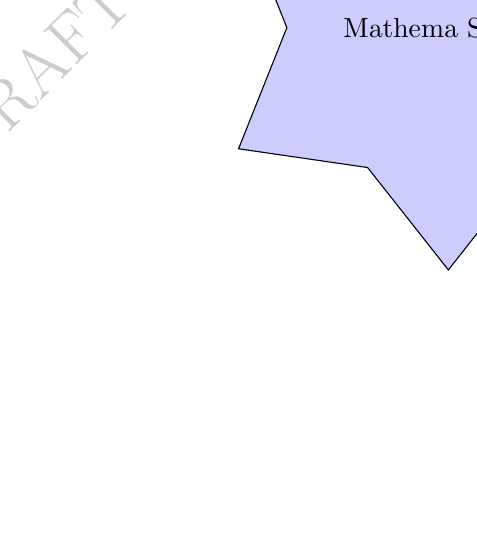
\begin{tikzpicture}
		\tikz \node [fill=blue!20,star,star points=6,draw] {Mathema Shukur };
	\end{tikzpicture}
	\\
	যাদের জন্যে প্রযোজ্যঃ  	\textcolor{magenta}{একাদশ ও দ্বাদশ শ্রেণীর শিক্ষার্থী} \\
	বিষয়ঃ \textcolor{magenta}{উচ্চতর গণিত ১ম পত্র} \\
	অধ্যায়ঃ \textcolor{magenta}{৩-সরলরেখা}\\ 
	Subtopicঃ  \textcolor{magenta}{ $ax+by+c=0$ এর সমান্তরাল রেখার সমীকরণ নির্ণয় কর }\\
	\\
	\textcolor{blue}{$ax+by+c=0$ এর সমান্তরাল রেখার সমীকরণ  $ax+by+k=0$}\\
	\\
	এ ক্ষেত্রে শুধুমাত্র ধ্রুবক পদ পরিবর্তিত হবে \\ 
	\\ 
	দিনাজপুরবোর্ড-২০২১\\ 
	$(1,0)$ বিন্দুগামী $2x+5y+1=0$ রেখার সমান্তরাল রেখার সমীকরণ নির্ণয় কর \\
	\\
\textcolor{red}{step-01}	$2x+5y+1=0$ রেখার সমান্তরাল রেখার সমীকরণ $2x+5y+k=0$\\
	\\
\textcolor{red}{step-02}	$2x+5y+k=0$ রেখাটি $(1,0)$ বিন্দুগামী \\
	\\
	\begin{align*}
	2x+5y+k&=0\\
	\\
	2(1)+5(0)+k&=0\\
	\\
	2+k&=0\\
	\\
	k&=-2
	\end{align*}
\\
	$2x+5y+1=0$ রেখার সমান্তরাল রেখার সমীকরণ $2x+5y-2=0$\\
		\\
	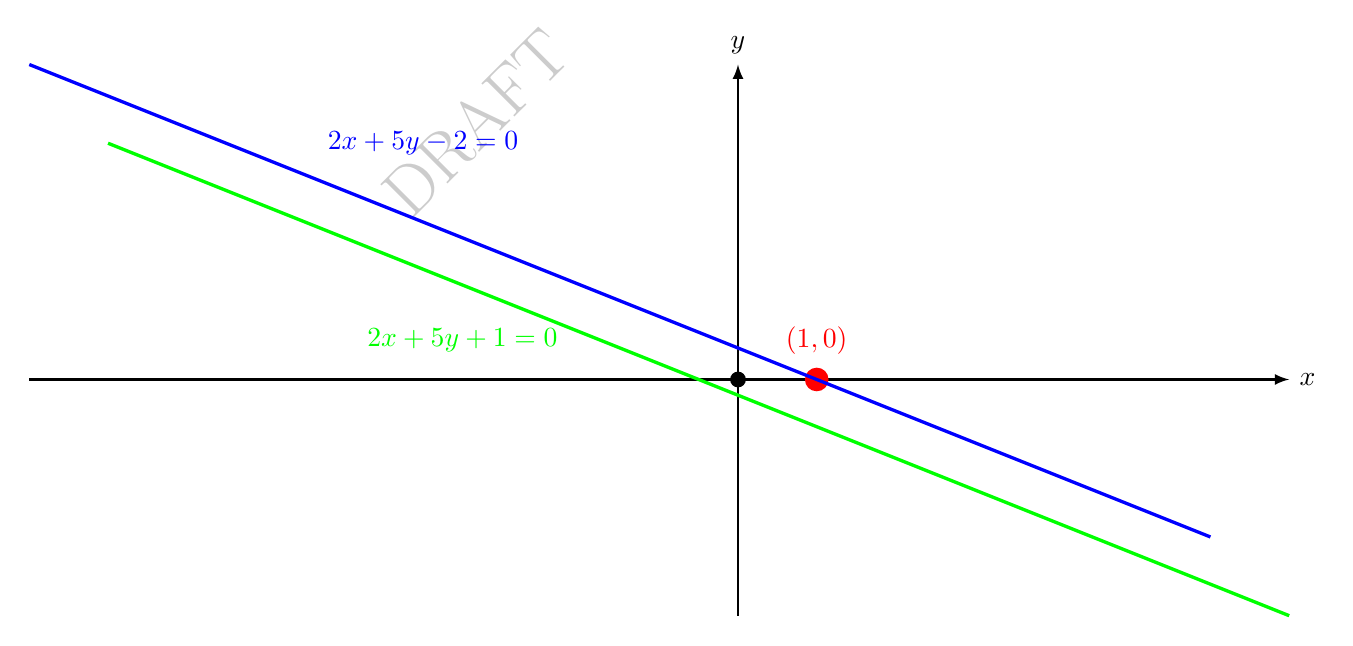
\begin{tikzpicture}[transform shape,scale=1]
		\draw [-latex,thick](-9,0) -- (7,0) node[right] {$x$} coordinate(x axis);
		\draw [-latex,thick](0,-3) -- (0,4) node[above] {$y$} coordinate(y axis);
		\fill[black] (0,0) circle (1 mm);
			\fill[red] (1,0) circle (1.5 mm);
		\node at (-4,3) {$\textcolor{blue}{2x+5y-2=0}$};	
		\node at (-3.5,0.5) {$\textcolor{green}{2x+5y+1=0}$};	
			\node at (1,0.5) {$\textcolor{red}{(1,0)}$};	
		\draw[very thick,green] (-8,3)--(7,-3);	
		\draw[very thick,blue] (-9,4)--(6,-2);	
	\end{tikzpicture}
	\\
	\textcolor{red}{$ax+by+c=0$ সরলরেখার  সমান্তরাল সরলরেখা যা $(\alpha, \beta )$ বিন্দুগামী এরুপ সরলরেখার সমীকরণ  $ax+by=a\alpha+b\beta$}\\
	\\ 
	ময়মনসিংহ বোর্ড-২০২১\\
		$(1,-2)$ বিন্দুগামী $12x+5y-3=0$ রেখার সমান্তরাল রেখার সমীকরণ নির্ণয় কর \\
		\\ 
	\textcolor{red}{single step}	$12x+5y-3=0$ সরলরেখার  সমান্তরাল সরলরেখা যা $(1,-2)$ বিন্দুগামী এরুপ সরলরেখার সমীকরণ \\
		\\
		 $12x+5y=12(1)+5(-2)=2$\\
		\\
		$12x+5y=2$\\
		\\
	\begin{tikzpicture}[transform shape,scale=1]
		\draw [-latex,thick](-4,0) -- (6,0) node[right] {$x$} coordinate(x axis);
		\draw [-latex,thick](0,-6) -- (0,13) node[above] {$y$} coordinate(y axis);
		\fill[black] (0,0) circle (1 mm);
		\node at (-2,4) {$\textcolor{blue}{12x+5y-2=0}$};	
		\node at (4.5,0.5) {$\textcolor{green}{12x+5y-3=0}$};	
		\draw[very thick,green] (5,-6)--(-3,13);	
		\draw[very thick,blue] (5,-8)--(-3,11);	
	\end{tikzpicture}
\\
	$(1,-2)$ বিন্দুগামী $12x+5y-3=0$ রেখার সমান্তরাল রেখার সমীকরণ 	$12x+5y-2=0$
\end{document}